\section{Bevor es losgehen kann - PC und Smartphone einrichten} \label{Bevor es losgehen kann}
Bevor es mit der eigentlichen Programmierarbeit losgehen kann, muss zuerst das schon erw\"ahnte Android \ac{SDK} von der Google-Developer-Seite \footnote{\url{http://developer.android.com/sdk/index.html}} heruntergeladen und installiert werden. Ist dies erledigt, kann es eigentlich schon fast losgehen.

\subsection{Der Android SDK Manager} \label{Der Android SDK Manager}
Bevor die Programmierarbeit starten kann muss, nach der Installation, zuerst der "`Android SDK Manager"' gestartet werden. Dies ist zum einen wichtig, um die neusten Updates zu bekommen, aber auch um die passenden APIs, welche Verwendung finden sollen, herunterzuladen.

Der Android \ac{SDK} Manager kann entwerder aus der \ac{IDE} (siehe Kapitel \ref{Die Eclipse IDE mit dem ADT Plugin}) oder direkt im Installationsverzeichnis unter \texttt{/sdk/tools/android} gestartet werden.

Wie schon erw�hnt, ist der Manager zum einen die Update-Plattform des \ac{SDK}-Pakets und zum anderen auch der Installer f�r neue Pakete.

Beim Starten des \ac{SDK} Managers werden, soweit verf\"ugbar, neue Updates f�r schon installierte Pakete angeboten. Damit der Download und die Installation startet, muss der Nutzer diesen Vorgang best�tigen. Sind alle Updates geladen und werden keine neuen Pakete ben�tigt, kann der Manager wieder geschlossen werden.

Beim ersten Starten der \ac{IDE} und des Managers muss ausgew�hlt werden, auf welchem API-Level (welcher Android-Version) programmiert werden soll. Da Android relativ weit abw�rtskompatibel ist, empfiehlt es sich bei einem neuen Projekt immer die neuste API zu installieren und diese auch zu verwenden.  

Durch die Verwendung der neuesten API ist zum einen garantiert, dass das Projekt auf der neuesten Android-Version l\"auft, zum anderen ist sichergestellt, dass das Projekt relativ lange ohne \"Anderungen mit zuk\"unftigen API-Versionen lauff\"ahig bleibt.

Wurde eine API geladen, kann die Programmierarbeit in der \ac{IDE} begonnen werden.

\subsection{Die Eclipse \ac{IDE} mit dem \ac{ADT} Plugin} \label{Die Eclipse IDE mit dem ADT Plugin}
% Falls bei ersten Start unter Ubuntu der Fehler: \texttt{error while loading shared libraries: \\libstdc++.so.6: cannot open shared object file: No such file or directory}

Im Bild \ref{Eclipse_IDE} ist ein Screenshot der Eclipse \ac{IDE} mit dem installierten \ac{ADT}-Plugin zu sehen, wie es nach der Installation vom \ac{SDK} aussieht.
F\"ur die Bearbeitung dieser Arbeit wird die monentan aktuelle \ac{SDK}-Version "`20140702"', welche auf Eclipse Juno basiert, eingesetzt.

Im oberen Teil ist die Steuerleite zu finden, \"uber deren Button zum Beispiel ein Debug durchgef\"uhrt oder das aktuelle App-Projekt gestartet werden kann. Hier sind des Weiteren auch Buttons zum Starten des \ac{SDK}-Managers, die Virtual-Device-Auswahl oder der Button f\"ur die Deaktivierung der "`Breakpoints"' zu finden.

Im linken Abschnitt des Fensters ist, der in Eclipse \"ubliche, Projektbaum (Projektexplorer) zu finden, welcher die vorhandenen Projekte anzeigt. Im Bild sind zwei Projekte zu sehen, welche im Abschnitt \ref{Ein Projekt Anlegen} genauer geschrieben werden. 

Im mittleren Teilfenster, der IDE, ist der eigentliche Editor f\"ur den Quellcode zu sehen. In der Abbildung \ref{Eclipse_IDE} ist die, im Projektbaum markierte, Datei \texttt{MainActivity.java}, im Editor, dargestellt.

Der rechte Teil des Fensters stellt die im Editor angezeigte Klasse beziehungsweise Datei schematisch dar. Hier sind unter dem Klassennamen alle Methoden und klassenweite Instanzen zu sehen. \"Uber einen Klick auf ein Element springt der Editor zur gew\"ahlten Methode beziehungsweise Variable.

Im unteren Bereich ist zum einen die Problem-Ansicht von Eclipse, die Konsole und die "`LogCat"' zu finden. Bei der LogCat handelt es sich um eine Debuganzeige, welche Warnungen, Fehler und Informationen im Android-Betriebssystem anzeigt. Wie die LogCat zu benutzen ist und wie eine Anzeige innerhalb einer App generiert wird, wird im Kapitel \ref{Die LogCat} genauer beschrieben.

\begin{figure}[!ht]
\centering
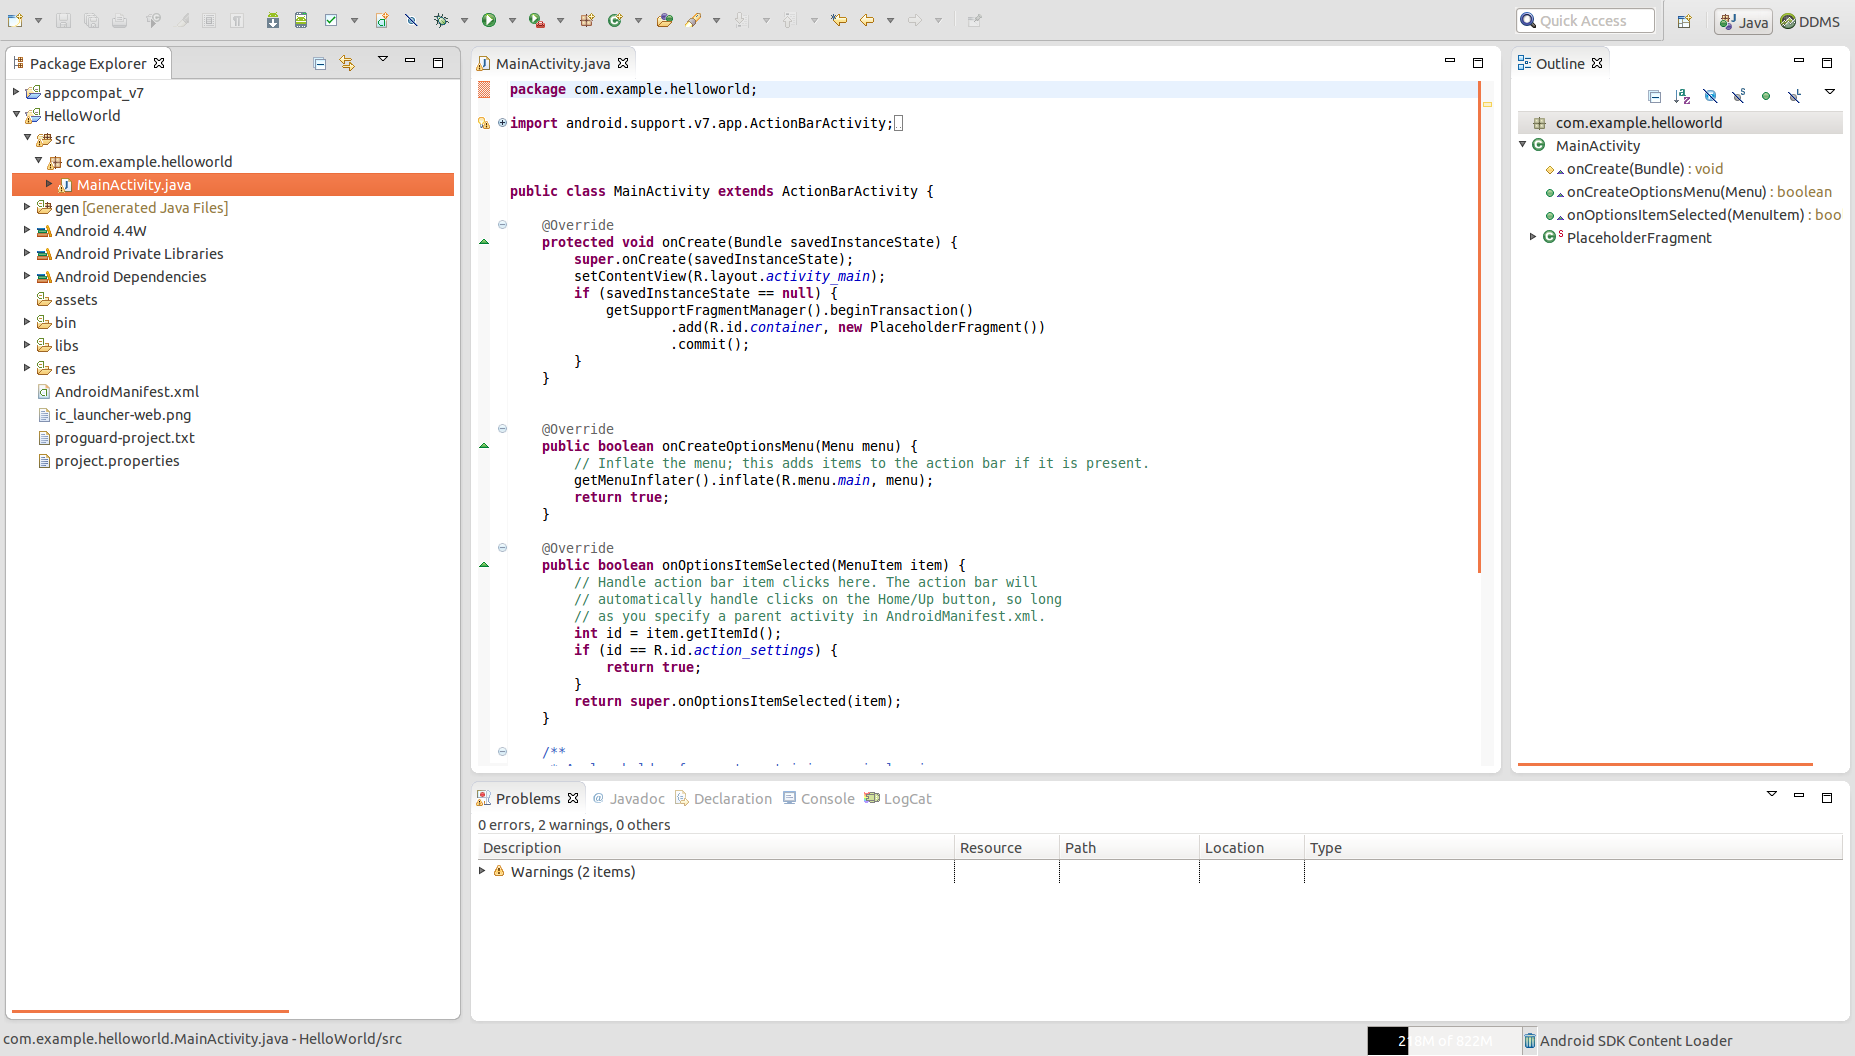
\includegraphics[width=16cm]{Bilder/IDE_Screenshut.png}
\caption{Die Eclipse \ac{IDE} mit dem \ac{ADT}-Plugin}
\label{Eclipse_IDE}
\centering
\end{figure}

Damit das \ac{ADT}-Plugin unter Ubuntu eigesetzt werden kann, m\"ussen drei zus\"atzliche Bibliotheken nachgeladen werden. Dies ist mit dem folgenden Konsolenbefehl m\"oglich:
\lstinputlisting{Code/libInstall.sh}

Sollten diese Biblioteken noch nicht im System vorhanden sein, so wird beim Start der \ac{IDE} der Fehler \texttt{error while loading shared libraries: \\libstdc++.so.6: cannot open shared object file: No such file or directory} ausgegeben.

\subsubsection{Ein Projekt anlegen} \label{Ein Projekt Anlegen}
Um eine App zu programmieren, wird ein Projekt ben\"otigt, welches mit Hilfe eines Wizards erzeugt werden kann. Mit einem Rechtsklick im Projektexplorer \"offnet sich das Kontextmen\"u wo unter "`Neu"' verschiedene Wizards zur Auswahl stehen.
Nun muss f\"ur ein neues Projekt "`Android Application Project"' gew\"ahlt werden. \"Uber den somit aufgerufenen Wizard ist es m\"oglich die grundlegende Projektstruktur zu erstellen. Hierf\"ur m\"ussen grundlegende Einstellungen wie der Projektname, der Packagepfad und ein Icon angegeben werden.

Wird dem Wizard in der Standardkonfiguration gefolgt, wird eine "`Hello World"'-App erstellt, welche den Text "`Hello World"' am Bildschirm ausgibt. \cite{Kuehn12}

Nach dem Anlegen sind zwei Projekte im Verzeichnis zu finden. Zum einen das "`HelloWorld"'-Projekt, welches die App enth\"alt und zum anderen ein Projekt mit dem Namen "`appcompat\_v7"', welches die f\"ur ein Projekt ben\"otigten Librarys enth\"alt. Das HelloWorld-Projekt verweist auf die, automatisch erstellten, Projekt-Librarys von appcompat\_v7. Dies ist sinnvoll, da bei einem API-Wechsel gegebenenfalls andere oder neue Librarys automatisch eingebunden werden.

\"Uber die Schaltfl\"ache mit dem Play-Symbol in der oberen IDE-Leiste kann die, eben erstellte, App gestart werden. Dies kann entweder mit dem Vitual Device oder auf realer Hardware gemacht werden.
% \newpage

\subsubsection{Eine App im Virtual Device ausf\"uhren}
\begin{wrapfigure}{r}{4,95cm}
\vspace{-13pt}
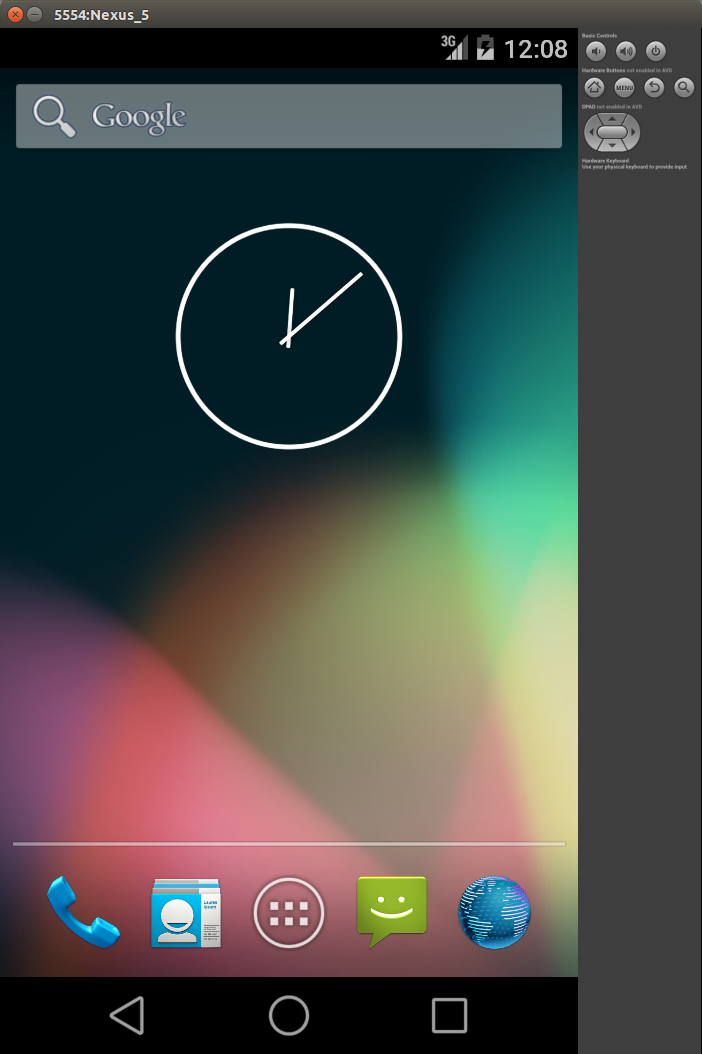
\includegraphics[width=4.95cm]{Bilder/VirtualDeviceScreenShot.png}
\caption{Android L Startbildschirm des Virtual Device}
\label{Startbildschirm des Virtual Device}
\vspace{-40pt}
\end{wrapfigure}

Nach dem Starten der App muss eine Auswahl getroffen werden, auf welchem Ger\"at die App installiert und gestartet werden soll.

Hierf\"ur muss einmalig ein Virtual Device mit der gew\"unschten Betriebssystem-Version erstellt werden. Au\ss{}erdem besteht die M\"oglichkeit, reale Ger\"ate, wie ein Nexus 5 nicht nur in der Prozessor- und Arbeitsspeicherleistung sondern auch dessen Bildschirmgr\"o\ss{}e und Aufl\"osung zu simulieren. \cite{GolemHBEmulator}

Wurde ein Virtual Device gew\"ahlt, wird die Virtualisierung des Ger\"ates gestartet und die erstellte App darauf installiert.

Um das Betriebssystem des Virtual Device nicht immer fortw\"ahrend neu zu starten, empfiehlt es sich, beim Erstellen den Check-Punkt "`Snapshot"' anzuhaken. Hierdurch wird beim schlie\ss{}en des Virtual Device der aktuelle Zustand gespeichert und beim n\"achsten Ausf\"uhren aufgerufen. Dies hat den Vorteil, dass das Device nicht erst starten muss und somit schneller einsatzbereit ist. \cite{VirtualDeviceErstellen}

Sollen Services von Google wie zum Beispiel Google Maps in der App verwendet werden, muss ein Virtual Device mit Google APIs erstellt werden, wie dies funktioniert ist im Kapitel \ref{Google-APIs} genauer beschrieben. \cite{GolemHBGoogleServices}

\subsubsection{Eine App auf realer Hardware ausf\"uhren} \label{Eine App auf realer Hardware Ausfuhren}
Um eine App auf einem realen Androidger\"at ausf\"uhren zu k\"onnen, muss in diesem die Entwickleroption freigeschaltet werden. Dies geschieht ,unter dem Nexus 5 mit purem Android 4.4.4, im Hauptmen\"u unter Einstellungen. Im Men\"upunkt "`\"Uber das Telefon"' muss sieben mal auf die Build-Nummer getippt werden um die Entwickleroptionen freizuschalten. Dies ist notwendig da die Entwickleroptionen seit Android 4.2 standardm\"a\ss{}ig deaktiviert sind. Bei anderen herstellereigenen Version von Android kann dies jedoch auch deutlich abweichen.  \cite{EntwickleroptionenFreischaltenS4}

Ist das geschehen, ist im Einstellungsmen\"u unter System der Eintrag "`Entwickleroptionen"' sichtbar. Hier k\"onnen nun viele f\"ur die Entwicklung wichtige Einstellungen vorgenommen werden. \cite{EntwickleroptionenFreischalten}

Um eine App von der IDE aus auf ein Ger\"at zu \"ubertragen, muss der Eintrag "`USB-Debugging"' unter Entwickleroptionen aktiviert werden. Ist dies geschehen, muss das Ger\"at per USB-Kabel an den Entwicklungsrechner mit der IDE angeschlossen werden, um eine App darauf zu installieren und zu debuggen. \cite{GolemHBEntwickleroptionen}

Wird das Ger\"at zum ersten mal angeschlossen, fordert es eine Best\"atigung um Apps, von dieser Quelle, installieren zu k\"onnen. Diese Meldung muss best\"atigt werden, damit Eclipse die App auf das Ger\"at \"ubertragen, starten und debuggen kann.

Wird nun die Play-Schaltfl\"ache bet\"atigt, fragt die IDE, bei angeschlossenen Ger\"at, ob es die App auf der realen Hardware oder im Virtual Device starten soll.

\subsection{Eine APK-Datei} \label{Eine APK-Datei}
Wird ein Projekt kompiliert, so wird vom \ac{SDK} eine .apk-Datei erstellt, welche die eigentliche App darstellt. Diese Datei ist im \texttt{bin}-Ordner des Projektverzeichnisses abgelegt und nicht f\"ur eine Weitergabe vorgesehen. 

Eine .apk-Datei ist eine Art komprimierter Zip-Ordner, welcher das Android-Manifest, den kompilierten Quellcode und alle verwendeten Ressourcen und Bibliotheken enth\"alt.

Damit eine App auf einem Androidger\"at installiert werden kann, muss sie mit einem digitalen Zertifikat versehen werden. F\"ur den Debug-Betrieb legt das \ac{SDK} standardm\"a\ss{}ig einen Debug-Key an, mit dem die App zertifiziert wird. Nur eine mit dem entsprechenden Debug-Zertifikat versehene App kann auf der f\"ur den Debug eingerichteten Hardware laufen.

\subsection{Die LogCat} \label{Die LogCat}
Bei der LogCat handelt es sich um ein Logging-Tool, welches jederzeit in Android aktiv ist und Log-Ausgaben von allen Apps und dem Betriebssystem sammelt. Jede Applikation kann Informationen in das Log schreiben, wobei die Menge der Log-Zeilen vom Programmierer abh\"angig ist, da er selbst bestimmt, welche Informationen er in das Log schreibt.

Die LogCat ist als Ringpufferspeicher realisiert und hat zum Beispiel beim Samsung Galaxy Note eine gr\"o\ss{}e von 800KB. Als Standard f\"ur die Speichergr\"o\ss{}e gibt Google jedoch nur 64KB an. Hier l\"asst sich gut erkennen, das viele Einstellungen im Betriebssystem von den Hardwareherstellern festgelegt werden.

Da es sich bei der LogCat um einen Ringpufferspeicher handelt, werden die \"altesten Daten automatisch \"uberschrieben. Somit ist die Speicherdauer davon abh\"angig, wie viele Log-Eintr\"age in einer bestimmten Zeit gemacht werden. \cite{LogCat}

Wird ein Ger\"at an den Entwicklungsrechner angeschlossen, so wird automatisch der gesammte Ringpufferspeicher der LogCat in die \ac{IDE} \"ubertragen und in der LogCat angezeigt.

Die LogCat ist in der Lage die Ausgaben Verbose, Debug, Information, Warning und Error zu unterscheiden. Hierf\"ur stehen in der Android-API verschiedene Methoden zur Verf\"ugung.

Um die LogCat Eintr\"age in der LogCat vorzunehmen, muss im Programmcode die Klasse \texttt{Log} verwendet werden. Diese hat die Methoden \texttt{v}, \texttt{d}, \texttt{i}, \texttt{w} und \texttt{e}, welche im Listing aufgef\"uhrt sind.

\lstinputlisting{Code/LogCatMethoden.java}

Der als "`TAG"' bezeichnete String-Parameter in den Methoden sollte den Klassennamen, in der die Log-Ausgabe gemacht wird, enthalten.
Google schl\"agt hierf\"ur in der Klasse eine Konstante TAG vor, welche den Klassennamen enth\"alt. \cite{APILog}

Die eben beschiebenen Mehoden sind alle \"uberladen und k\"onnen jeweils noch einen weiteren Parameter aufnehmen. Dieser Parameter erlaubt es eine Java Exception direkt in der LogCat auszugeben.

Google schl\"agt in seinen APIs vor, die beschriebene Konstante \texttt{TAG} wie folgt zu Implementieren.

\lstinputlisting{Code/GoogleLogCatConstante.java}

Um Schreibfehler zu vermeiden, bietet es sich jedoch an, eine andere Variante zu verwenden.

\lstinputlisting{Code/KuehnLogCatConstante.java}

